\begin{figure}\centering
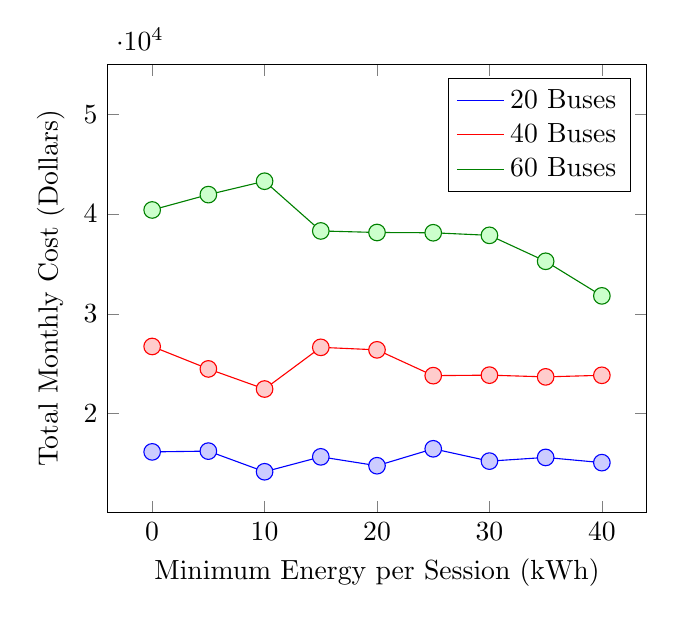
\begin{tikzpicture}
\begin{axis}[xlabel=Minimum Energy per Session (kWh), ylabel=Total Monthly Cost (Dollars), ymax=55000, legend pos=north east]
	\addplot[blue] coordinates {
		(0, 16183.79)   
	  (5, 16260.98)  
		(10,14194.10)  
		(15,15686.16)  
		(20,14798.53)  
		(25,16492.56)  
		(30,15259.19)  
		(35,15628.38)  
		(40,15106.82)};
\addplot[red] coordinates {
		(0, 26738.71)
		(5, 24491.03)
	  (10,22476.88)
		(15,26650.71)
		(20,26400.31)
		(25,23816.91)
		(30,23866.55)
		(35,23693.25)
		(40,23851.78)};
\addplot[green!50!black] coordinates {
		(0, 40405.72)
		(5, 41942.45)
	  (10,43284.09)
		(15,38304.96)
		(20,38150.28)
		(25,38122.51)
		(30,37864.79)
		(35,35268.11)
		(40,31805.12)};

\addplot[blue!20, draw=blue, only marks, mark size=3pt] coordinates {
		(0, 16183.79)  
		(5, 16260.98)  
	  (10,14194.10)  
		(15,15686.16)  
		(20,14798.53)  
		(25,16492.56)  
		(30,15259.19)  
		(35,15628.38)   
		(40,15106.82)};
\addplot[red!20, draw=red, only marks, mark size=3pt] coordinates {
	(0, 26738.71)  	
	(5, 24491.03)  	
	(10,22476.88)   
	(15,26650.71)  	
	(20,26400.31)  	
	(25,23816.91)  	
	(30,23866.55)  	
	(35,23693.25)  	
	(40,23851.78)};	
\addplot[green!20, draw=green!50!black, only marks, mark size=3pt] coordinates {
	(0, 40405.72)  
	(5, 41942.45)  
	(10,43284.09)  
	(15,38304.96)  
	(20,38150.28)  
	(25,38122.51)  
	(30,37864.79)  
	(35,35268.11)  
	(40,31805.12)};

\legend{20 Buses, 40 Buses, 60 Buses} 
\end{axis}
\end{tikzpicture}
\caption{Cost comparison of different degragmentation thresholds in a pro-time optimization scheme.}
\label{fig:results:defragmentationCostProTime}
\end{figure}
